\documentclass{article}
\usepackage{tikz}
\usetikzlibrary{positioning}
\begin{document}

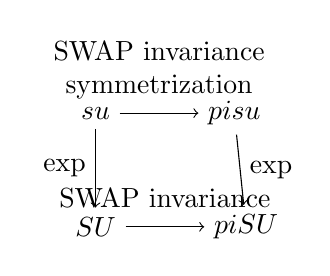
\begin{tikzpicture}
  \node (su) {$\mathfrak{su}$};
  \node[right=of su] (pisu) {$\operatorname{pi}\mathfrak{su}$};
  \node[below=of su] (suU) {$SU$};
  \node[right=of suU] (pisuU) {$\operatorname{pi}SU$};
  \draw[->] (su) -- node[above] {\begin{tabular}{c}SWAP invariance\\symmetrization\end{tabular}} (pisu);
  \draw[->] (suU) -- node[above] {\begin{tabular}{c}SWAP invariance\\\end{tabular}} (pisuU);
  \draw[->] (su) -- node[left] {exp} (suU);
  \draw[->] (pisu) -- node[right] {exp} (pisuU);
\end{tikzpicture}

\end{document}